\documentclass[a4paper, 10pt, conference]{ieeeconf}
\usepackage[utf8]{inputenc}
\usepackage{amsmath}
\usepackage{graphicx}
\usepackage{pgf-pie}
\usepackage{tikz}
\usepackage[hidelinks]{hyperref}
\usetikzlibrary{positioning,shadows,arrows,backgrounds}

\usepackage{xcolor}
\newcommand\todo[1]{\textcolor{red}{\textbf{TODO}: [#1]}}

\IEEEoverridecommandlockouts
\overrideIEEEmargins

\title{\LARGE \bf
Stegos  -- a design for a private, confidential, and scalable cryptocurrency}
\author{Vladimir Lebedev, David McClain\\Stegos AG, October 2018}%

\begin{document}

\maketitle
\thispagestyle{empty}
\pagestyle{plain}

%%%%%%%%%%%%%%%%%%%%%%%%%%%%%%%%%%%%%%%%%%%%%%%%%%%%

\begin{abstract}
    On October 31\textsuperscript{st} 2008, a person or group named ‘Satoshi Nakamoto’ released a paper called ``Bitcoin: A Peer-to-Peer Electronic Cash System.''\cite{c1} In the ten years since that paper was published, Bitcoin has become the most-used cryptocurrency in the world and inspired many researchers and developers to create their own blockchains that build and improve upon Bitcoin and its ideas.
    
    One of these areas of improvement is privacy --- while it is true that payments in Bitcoin are conducted between pseudonymous users, the payment transactions are stored in a public decentralized ledger from which a lot of information can be deduced. At the time of writing, there are more than a dozen \textit{privacy coins}, each using sophisticated algorithms to protect their users' privacy. However, they all have substantial drawbacks. 
    
    Some privacy coins protect identities of senders and recipients, but keep transaction amounts public. Few existing privacy coins can scale, because their ledgers are ever-growing and cannot be compacted. Most of these coins use proof-of-work consensus, which wastes enormous amounts of electricity and harms the environment. 
    
    In this paper, we propose a design for a private, confidential, and scalable blockchain that is environmentally friendly. Our design builds and improves upon other privacy coins and can be used to send payments and data with complete confidentiality. 
\end{abstract}

\section{Introduction}
This section provides a brief overview of the most prominent privacy coins and analyzes their privacy-protecting and performance characteristics.

We also explain how Stegos builds and improves on existing privacy coin ideas and employs the latest research into cryptography and blockchains to create a privacy-preserving blockchain that can be scaled. 

\subsection{Terminology}
We begin by defining various terms that are used throughout this paper:

\begin{itemize}
	\item \textbf{Privacy}: protection of the identity of blockchain participants and parties to transactions from detection.
	\item \textbf{Confidentiality}: protection from analyzing blockchain data (e.g., transaction details, including amounts) by unauthorized third parties.
	\item \textbf{Unlinkability}: for any two outgoing transactions, it is impossible to prove whether they were sent to the same person\cite{c2}.
	\item \textbf{Untraceability}: for each incoming transaction, all possible senders are equiprobable\cite{c2}.
	\item \textbf{Compactness}: spent coins can be pruned from the blockchain and the blockchain can be compacted.
	\item \textbf{Sharding}: a transaction verification and block-sealing process that can be partitioned between participants or groups of participants.
	\item \textbf{Interactivity}: senders and recipients of transactions must interact with each other \textit{off-chain} before posting a transaction to the blockchain.
	\item \textbf{Trusted Setup}: blockchain participants must trust someone to generate and then destroy some initial parameters.
	\item \textbf{PoW (proof of work)}: an original consensus protocol for Bitcoin, where each node participating in the protocol must present a piece of data which is difficult (costly, time-consuming) to produce but easy for others to verify and which satisfies certain requirements. Due to the complexity of the computations and the number of miners, the Bitcoin PoW consensus currently consumes approximately 73TWh of electricity per year\footnote{https://digiconomist.net/bitcoin-energy-consumption}.
	\item \textbf{PoS (proof of stake)}: a consensus algorithm where the creator of the next block is chosen via various combinations of random selection, wealth, age and staked funds. PoS blockchains can be more energy efficient than currencies based on PoW algorithms\footnote{http://cfa-consulting.ch/dlfiles/NxtEnergyandCostEfficiencyAnalysis.pdf}.
	\item \textbf{UTXO (unspent transaction output)}: a transaction output that can be spent as an input in a new transaction.
\end{itemize}

\subsection{Existing privacy coins}

\subsubsection{Monero} originated as a Bytecoin fork in 2014 under the name Bitmonero. Monero uses a UTXO model and PoW consensus and is based on the CryptoNote protocol\cite{c2}, employing the ring signatures method. In 2017, Monero implemented RingCT\cite{c3}, an improved version of the ring signatures. RingCT enables confidentiality of amounts and untraceability of transactions. In combination with stealth addresses (also introduced in the original CryptoNote paper), which provide unlinkability of recipients, this provides full privacy and confidentiality.

Monero's blockchain cannot be compacted because spent UTXOs cannot be pruned from it. Keeping all UTXOs forever is one of the requirements of RingCT protocol, which obfuscates the fact that particular UTXOs mentioned in transaction inputs have actually been spent. 
The recent introduction of Bulletproofs\cite{c4} to replace Monero's original zero-knowledge range proofs has reduced the basic transaction size from 13KB to 2.5KB, but the problem of ever-growing blockchains cannot be solved. 

\subsubsection{ZCash} originated in 2016 as a Bitcoin fork and therefore uses a UTXO model and PoW consensus. Zcash aims to correct the flaws of Bitcoin, with a focus on privacy. The project is building on work done on Zerocoin\cite{c5} by addressing some of its faults, particularly the size of the proofs, which ZCash decreases to 1KB, and speeding up verification.

To establish confidentiality and untraceability, ZCash implements ``Zero-Knowledge Succinct Non-Interactive Argument of Knowledge'' (zk-SNARKs)\cite{c6}. To provide unlinkability of recipients, ZCash employs stealth addresses.

zk-SNARKs enable a large anonymity set of all minted coins\footnote{The \textit{anonymity set} is defined as the set of participants who could be a sender in ZCash transaction, as seen by a global observer who has also compromised a set of nodes.}, providing a high degree of privacy. However, with an average transaction size of up to 2KB and an ever-growing an unprunable accumulator which holds the serial numbers of all spent coins, ZCash is unscalable in the long run. This scalability issue is the main reason why privacy is currently optional when using ZCash. At the time of writing, less than 25\% of all transactions were shielded.

The questionable part of the zk-SNARKs protocol is the initial trusted setup. ZCash utilizes a multi-party ceremony involving several trusted people. This is controversial, as users must trust that the ceremony was carried out correctly and that the trusted parties destroyed their initial parameters as claimed. 

\subsubsection{Dash} originally a codebase fork of Litecoin (which is in turn a codebase fork of Bitcoin), Dash was launched as XCoin in January 2014. Dash uses the UTXO model and PoW consensus. 

In addition to standard nodes and miners, Dash has \textit{masternodes}. These nodes  must have static IP address and fulfill particular requirements for CPU, RAM, and disk space. Each masternode must have at least 1000DASH in its ownership. A proof-of-service protocol ensures that masternodes have the most current blockchain protocol and are online. 

It is important to note that privacy is optional in Dash and the high volume of transactions is driven mainly by fast public transactions called \textit{InstantSend} which are provided by masternodes.

\textit{PrivateSend} is an implementation of CoinJoin, the untraceability solution first proposed for Bitcoin by Bitcoin Core developer Gregory Maxwell.\footnote{https://bitcointalk.org/index.php?topic=279249.0} In PrivateSend, three users add their coins together in a single combined transaction that sends the coins to freshly generated addresses belonging to the same three users. As such, the coins are effectively mixed between the three participants, breaking the blockchain trail of ownership between them. This process can be automatically repeated up to eight times, with (hopefully) different mixing participants, for extra privacy.

Dash does not provide confidentiality of amounts in either InstantSend or PrivateSend. In addition, the CoinJoin protocol requires that the inputs of users involved in each round of the mixing protocol have identical denominations (amount of coins). This requirement is impossible to fulfill if amounts are cloaked. 

Users of Dash must trust that masternodes will keep users' IP addresses undisclosed and unlinked to users' UTXOs when sending transactions, which adds another privacy vulnerability to Dash.

\subsubsection{Mimblewimble (Grin)} is a protocol proposed in a Bitcoin developers' chat room by an anonymous user under the name Tom Elvis Jedusor, who left a link to a paper\footnote{https://download.wpsoftware.net/bitcoin/wizardry/mimblewimble.txt} outlining the Mimblewimble protocol, a way to significantly enhance the scalability and privacy of the Bitcoin network.

Mimblewimble is based on ideas from Greg Maxwell's design for confidential transactions\footnote{https://people.xiph.org/\texttt{\~{}}greg/confidential\_values.txt}, except the recipient is the one who generates a random blinding factor used to cloak the amount of the transaction. This blinding factor is then used as proof of ownership by the recipient, therefore working simultaneously as the recipient's public key. In this way, Mimblewimble provides confidentiality of amounts and unlinkability of recipients in its transactions.

Untraceability of transactions in Mimblewimble is built on ideas from CoinJoin and is implemented by breaking transaction boundaries and storing only inputs and outputs of all transactions, verified by miners in a newly mined block.

The only currently known  implementation of the Mimblewimble protocol is the Grin project \footnote{https://github.com/mimblewimble/grin}, which has recently released the third iteration of their testnet. Grin uses the UTXO model and PoW consensus. Spent UTXOs in Grin can be pruned by recursively applying a simple pruning algorithm for each UTXO referenced in inputs of the newly mined block.

Despite these advantages, there are several drawbacks in the design of Mimblewimble and Grin:

\begin{itemize}
	\item {In order to create a transaction, the sender and recipient must interact with each other. A sender cannot post a transaction to the blockchain without first contacting the recipient with half-baked transaction data and receiving a response from the recipient updated using the blinding factor.}
	\item {Similar to the trust issue with Dash masternodes, Grin users must currently trust Grin miners that they will not trace the history of moving coin inputs to outputs in transactions, and will instead discard this data after mining a block. Since this cannot be guaranteed, there is therefore a potential threat to coin fungibility and user privacy.}
\end{itemize}

\subsection{Our contribution}
In this paper we propose a design for \textit{Stegos}, a blockchain which uses the \textit{UTXO} (coin) model and \textit{PoS} consensus.

Transactions in Stegos are \textit{unlinkable}, \textit{untraceable}, and \textit{confidential}:

\begin{itemize}
	\item {Stegos uses one-time payment addresses which make it impossible to identify recipients of a transaction (i.e., to link recipients' addresses to their identities), because all transactions are directed to new and unique addresses. The technique used for one-time addresses is very similar to that used for stealth addresses in Monero and ZCash.}
	\item {Stegos pools many individual transactions together to form super-transactions, making it impossible to trace the history of individual transactions. To achieve this, Stegos has adopted and enhanced the ValueShuffle protocol\cite{c7}, the first coin mixing protocol compatible with confidential transactions.}
	\item {All amounts in Stegos are hidden using Pedersen commitments\cite{c8} and Bulletproofs range proofs\cite{c4}. The only exceptions are validator stakes and transaction fees, since these must be visible for blockchain validation.}
\end{itemize}

Many projects claim to be able to process a million transactions per second (TPS), but none of them explain how they are going to maintain all the accumulated data. Bitcoin provides for 7--10 TPS, and the Bitcoin blockchain is expected to grow past 170GB by the end of 2018. If we assume that Bitcoin could suddenly support even 16,000 TPS, the Bitcoin blockchain would grow by 350 GB every day\footnote{https://hackernoon.com/if-we-lived-in-a-bitcoin-future-how-big-would-the-blockchain-have-to-be-bd07b282416f}, or 127 TB every year. This amount of data is completely unsustainable without centralizing the blockchain on a few supercomputers, something that runs contrary to blockchain’s decentralization ethos.

Stegos is a \textit{compact} blockchain. Spent coins are safely removed from the blockchain using secure cryptographic pruning. To keep our blockchain free from spent coins, we use the technique proposed by Satoshi Nakamoto in the original Bitcoin paper\cite{c1}.

Stegos uses transactional \textit{sharding} to scale. Separate groups of Stegos validators keep the whole blockchain state but verify only a subset of incoming transactions, using cross-shard atomic commits to eliminate double-spending. This scalability approach lets Stegos process hundreds of thousands of transactions per second.

Stegos is friendly to the environment and does not require terawatts of electricity to be spent mining blocks. Stegos uses PoS consensus, building on ideas of pBFT\cite{c9} and collective signing\cite{c10}\cite{c11}. Each new Stegos block must be verified and confirmed by a group of validators, all of which must put coins in escrow (their stake).

The value of the coins staked has a direct effect on each validator's probability of becoming a leader of the consensus and earning transaction fees. Stegos does not have block rewards, instead replacing them with the \textit{Jackpot}.

The Jackpot is a feature unique to Stegos, based on a familiar lottery concept. A portion of the fees from each block are added to the Jackpot, along with any stake forfeited by a validator caught cheating.

The Jackpot is distributed every few thousand blocks when validators run a cryptographic lottery based on verifiable distributed randomness. The amount in the Jackpot is then transferred to the winner. The longer a validator maintains their stake and participates in consensus, the higher the probability of winning the Jackpot lottery.

The consensus leader is elected and the Jackpot winner is chosen using our algorithm for generating distributed, untainted, unbiasable randomness, \textit{RandHound++}. RandHound++ is created in the spirit of the RandHound protocol\cite{c12}, although our algorithm actually derives much of its protocol from SCRAPE\cite{c13}. SCRAPE defines a PVSS\cite{c14} protocol using symmetric bilinear pairing based cryptography and coding theory. The algorithm has been further adjusted to deal with asymmetric pairings, which are needed to provide stronger cryptographic security.

The following sections explain each of the Stegos features presented above in more detail.

\section{Networking}\label{networking}

The Stegos network is composed of full nodes and light nodes (e.g., nodes running on mobile devices or browsers). Each full node maintains a full copy of the blockchain and associated data structures. Full nodes which put coins in escrow become \textit{validators} and may participate in the collective signing protocol (\textit{CoSi}) and respond to requests made by light nodes. 

Light nodes do not maintain the full blockchain; they only keep blockchain headers and know how to talk to validators. 

Stegos maintains the core of the network by running a number of validator nodes itself, known as \textit{core nodes}. This simplifies bootstrapping of new nodes and ensures network continuity. The addresses of these core nodes are hard-coded into each release of the Stegos blockchain software.

Nodes keep lists of addresses of the nodes they know about (peers), adding new peers as they become aware of them. A new node will begin by connecting to one of the core nodes to fetch a list of peers. Each full node quickly rebroadcasts received transactions to a set of its peers, after a few light checks. This ensures that node cannot be subject to a DDOS attack by spamming transactions to validate, and also that the node does not rebroadcast junk transactions.

To discourage bad actors, we employ a mechanism to both throttle peers and punish peers for bad transactions, etc., by blocking them from further participation in the network.

The Stegos blockchain uses gossip protocols to spread information without depending on fixed networks of communicating nodes. This protocol does not require every node to be reliable or always online, nor does it require every node to know about every other node. The key to a gossip protocol is that every node knows only a few other nodes (or even just one) in the network, but as long as most nodes know about at least two other nodes besides themselves, information can propagate through the network.

\section{Randomness}\label{randomness}

Bias-resistant distributed randomness is a critical component of Stegos. We employ \textit{RandHound++}, our improved variant of RandHound\cite{c12}, a large-scale distributed protocol that provides publicly verifiable, unpredictable, and unbiased randomness by implementing an efficient and decentralized randomness beacon. The protocol arranges participants into verifiably unbiased random secret-sharing groups, which repeatedly produce random output at predefined intervals. 

We use RandHound++ for multiple purposes:

\begin{itemize}
	\item {to form validator groups;}
	\item {to elect leaders of validator groups;} 
	\item {to choose facilitators for pooled transactions;}
	\item {to find a winner of the Jackpot lottery.}
\end{itemize}

\subsection{Distributed Randomness Generation}

Distributed randomness generation is based on having many nodes participate in the construction of an untainted and unpredictable random value in order to overcome Byzantine faults which might try to steer, or predict, the outcome.

RandHound++ is based on the notion of publicly verifiable secret sharing (PVSS)\cite{c15}, which ensures that every step of the process can be audited using zero-knowledge proofs (ZKPs), while keeping vital details of the process fully cloaked through strong cryptography.

Unlike distributed consensus protocols such as pBFT, we do not need full Byzantine threshold participation at every stage. In what follows we assume a maximum number, $f$, of faulty nodes, in a collection of $(3 f + 1)$ participant nodes. 

Standard BFT requires responses from a super-majority of $(2 f + 1)$ nodes in order to reach consensus. But generating randomness requires just $(f + 1)$ responses from participants to overcome any Byzantine faults, at least one participant will be honest and blend their randomness into the computation, ensuring the result is also truly random. 

We do not need consensus on the result as long as its process can be verified. It is sufficient to see that at least one node was honest, which is clearly true with $(f + 1)$ participants. Attackers can perturb the final value, but it will still be an honest random value by virtue of the inoculation property.

\subsection{RandHound++}

Our variant of the RandHound protocol is implemented with pairing-based cryptography (PBC). As such, it departs from the original RandHound algorithm in a number of significant ways. It is a distributed protocol for generating audit\-able, untainted, and unpredictable randomness, as required for fair stake-weighted elections of the validator group leader, among other thing.

After every election, a \textit{leader} is selected for each validator group, and a \textit{beacon} node is then chosen from among the remaining validators. The \textit{beacon} node is responsible for partitioning all validators (including itself and the leader) into RandHound++ groups. 

The first validator in any group becomes a {local group leader}. The local group leader collects randomness from all group members and itself, and then forwards that result back to the beacon. The beacon then combines all the group's randomness values into a single result that becomes the seed value for the next elections. The beacon then sends a \textit{HOLD-ELECTION} message with that seed value to all validators in the network.

A major advantage of PBC is that we can use efficient BLS signatures\cite{c16} in the protocol. Such signatures can be collectively added, along with the group sum of their public keys, to produce a short collective signature that can be validated just as easily as a single signature. BLS signatures are efficient because multi-signatures can be generated immediately and do not require a second query from participants in order to produce their collective signature.

However, using PBC introduces some complications in translating the RandHound algorithm to asymmetric pairs of elliptic curves. Though these complications are purely conceptual --- the mathematics are more difficult. 

In the near future we will publish a separate paper describing our improvements to the original RandHound protocol in more detail.

\section{Consensus}\label{consensus}

The Stegos consensus protocol is based on pBFT\cite{c9} but adds strong consistency. This allows all validators to agree on the validity of blocks without wasting computational power resolving inconsistencies. Clients do not need to wait more than a few seconds to be certain that a submitted transaction is committed; as soon as it appears in the blockchain, the transaction can be considered confirmed. 

\subsection{Collective Signing}

We adopt \textit{CoSi}\cite{c10}\cite{c11}, a scalable witness cosigning protocol which ensures that every authoritative statement is validated and publicly logged by a diverse group of witnesses before any client will accept it. A statement, $S$, collectively signed by $W$ witnesses assures clients that $S$ has been seen, and not immediately found erroneous, by those $W$ observers. Even if $S$ is compromised in a fashion not readily detectable by the witnesses, CoSi still guarantees $S$’s exposure to public scrutiny, forcing secrecy-minded attackers to risk that the compromise will soon be detected by one of the $W$ witnesses. 

CoSi builds on existing cryptographic multi-signature methods, scaling them to support thousands of witnesses via signature aggregation over efficient communications. The default implementation of CoSi uses Schnorr signatures, but we replace these with BLS signatures for performance reasons.

More details on using the CoSi protocol for sealing blocks in Stegos blockchain will be given later in this document, in Section \ref{tx_processing}.


\subsection{Leader Elections}

Stegos is a public decentralized blockchain, so anyone can join the network, become a validator, and earn rewards for maintaining it. Stegos uses PoS consensus, and all validators need to post a security bond of a fixed number of coins. Requiring a security bond helps prevent against Sybil attacks by requiring a significant financial commitment from each identity.

Any validator caught cheating by their peers loses their stake, which is added to the Jackpot. 

Validators elected to become a leader of the current epoch are rewarded by collecting transaction fees from the blocks they form.

Leader elections are carried out via stake-weighted lottery. The larger the validator stake (security bond), the greater the chances of winning the current round of the lottery. After serving one round, the leader relinquishes his right to be re-elected until some number of rounds later.

In order to produce a stake-weighted lottery, we imagine dividing a circle into angular sections proportional to individual stakes, with the full circumference of the circle representing the sum of all stakes. A uniformly generated random number over a finite interval (generated via our RandHound++ protocol) acts as a spinner in a dial readout, and wherever it points after a spin, that member is selected as the next leader. Larger stakeholders occupy a larger portion of the circumference, and so have a more likely chance of winning.

\begin{figure}[h!]
\centering

\resizebox{.3\textwidth}{!}{%

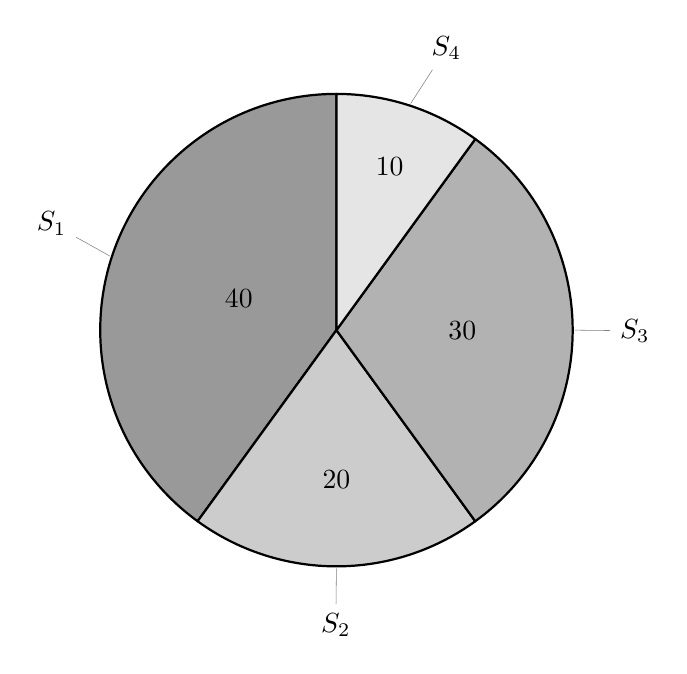
\begin{tikzpicture}
\pie [text=pin, rotate = 90, before number =, after number =,
	  color={black!40,black!20,black!30,black!10}]
	{40/$S_{1}$, 20/$S_2$, 30/$S_3$, 10/$S_4$}
\end{tikzpicture}

}%

\bigskip

\resizebox{.3\textwidth}{!}{%
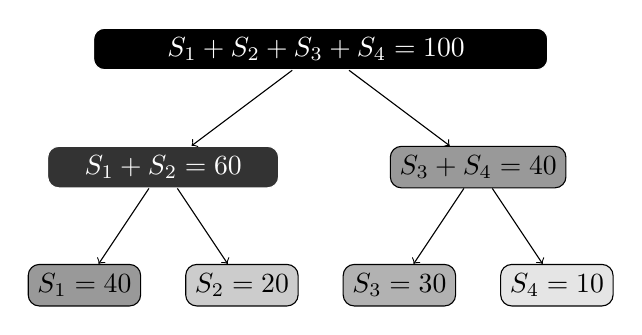
\begin{tikzpicture}[sibling distance=4cm,
  every node/.style = { shape=rectangle, rounded corners,
	draw, align=center, top color=white, bottom color=blue!20}]

\node[color=white, top color=black!100, bottom color=black!100]
	 {\ \ \ \ \ \ \ \( S_1 + S_2 + S_3 + S_4 = 100 \) \ \ \ \ \ \ \ }
	 child[->]
		  { node[color=white, top color=black!80, bottom color=black!80]
				{\ \ \ \( S_1 + S_2 = 60 \)\ \ \ }
				child[sibling distance=2cm]
					 { node[top color=black!40, bottom color=black!40] {\( S_1 = 40 \)}}
				child[sibling distance=2cm]
					 { node[top color=black!20, bottom color=black!20] {\( S_2 = 20 \)}}
		  }
	 child[->]
		  { node[top color=black!40, bottom color=black!40]
				{\(S_3 + S_4 = 40 \)}
				child[sibling distance=2cm]
					 { node[top color=black!30, bottom color=black!30] {\( S_3 = 30 \)}}
				child[sibling distance=2cm]
					 { node[top color=black!10, bottom color=black!10] {\( S_4 = 10 \)}}
		  };
\end{tikzpicture}
}%

\caption{Imagining a spin dial as a tree. Segments
are sized in proportion to the posted security bond (stake).}
  \label{fig:spinner}
\end{figure}

In practice, we form a binary tree of participants, in a consistent order, where each interior node represents the sum of all its sub-node stakes. The topmost node of the tree shows the full sum of all stakes represented in the tree, with all participants located in leaves. Branching decisions begin at the top node of the tree and descend toward leaves using the random value as a probe of the interval described by the partial sum at each node, with the division between left and right based on the relative weights of its two sub-trees. Descent continues until a leaf node is met, with that node declared the winner of the election. 

If the random probe value is converted into a fractional value of its range, and each interior node is relabeled with its division fractional value, then it is simple to choose left or right sub-nodes based on a single comparison between the two fractional values.

That this works can be seen by noting that every interior node of the tree serves as both denominator to nodes below and numerator to connections above, hence cancelling out. The final probability of any particular participant winning is therefore the same as their escrow stake divided by the sum of all participant escrow stakes.

\subsubsection{Handling leader failures} Leader elections are held on a schedule, and validators recognize the signal to hold a new election. 

The list of validators is publicly known and can be rebuilt by processing staking transactions, starting with the genesis block. Validators keep a number of data structures in memory, including the list of other validators, and update these data structures when accepting blocks to add to the end of the chain.

Each validator can re-run the election for themselves upon seeing the random value of the election signal, which arrives via the RandHound++ protocol. All nodes should therefore be able to agree on election outcome; however, if they cannot, then one of two things can happen: 

\begin{itemize}
	\item{First, if a validator thinks it has won the election but was mistaken, then any attempts at forming new CoSi networks by the faux leader will be silently rejected by the other validators, and it will fail to obtain a consensus on any new requests. If that happens, the rejected leader will resynchronize its list of validators, rerun its own election, and rejoin after agreeing on the outcome.} 
	\item{Second, a validator may think that someone else has won the election. In that case, it will silently reject signing requests by the actual election winner and never see any requests from the presumed one. The validator will re-sync its list of other validators if this happens for two consecutive election rounds.}
\end{itemize}

If the election winner is absent or comes under attack, it may not respond to its own election as leader, form a block, or broadcast a block for signing. Any validator can call for a new early election, and after $(2 f+1)$ (a super-majority) of such calls have been seen from different validators, a new election round will start.

\subsubsection{A fault-tolerant and self-healing protocol} Immediately after each leader election, each validator should determine its role for the new epoch:

\begin{itemize}
	\item If the node is elected leader, it should begin assembling the next block. 
	\item If the node becomes a member of a RandHound++ group, it should start running the protocol within its group.
	\item If the node becomes a facilitator for the transaction pooling protocol, it should start collecting transaction intent messages.
	\item If the node becomes a CoSi witness node, it should start a timeout timer. If the timeout ever fires, it is time to call for a new election. Incoming messages can restart or cancel the timeout timer.
	\item Otherwise, the node is on standby for the next election cycle. Nodes on standby can ignore almost all messages, but must pay attention to election-related messages.
\end{itemize}  

All validators should pay attention to leader election messages:

\begin{itemize}
	\item{\textit{New Election Message}: run an election with the random value provided in the election message, and determine the next role for this validator --- one of leader, witness signer, RandHound++ participant, facilitator, or standby. Reset the counter of calls for a new election.}
	\item{\textit{Call For New Election Message}: Increment the count, $n$, of such calls seen from different validators, and if $n \ge 2 f +1$, then run another election round based on the last election's random value, with a decision tree that excludes the current leader. Determine the new leader and the next role for this validator. Reset the counter of calls for a new election.}
\end{itemize}

\subsection{Key Blocks}

The Stegos blockchain is able to accommodate multiple types of blocks. The type of the block is defined by the \textit{Block Type ID} slot in the block header. In this paper we define two types of blocks: $0 (KeyBlock)$ and $1 (MonetaryBlock)$.

Monetary blocks --- the blocks that carry all cryptocurrency transaction data and coins --- will be described in detail in Section \ref{block}. These are referred to simply as \textit{blocks} throughout this paper. 

Key blocks are designed to deliver administrative information to blockchain participants. Any node which searches through key blocks can see the leader and witnesses (validators) for the current or past epoch. Nodes wishing to submit a transaction should consult the latest key block to find the current pooled transaction facilitator.

The key block header is constructed by the current leader filling in the following slots:

\begin{itemize}
	\item {Block Type ID, 0}
	\item {Version Number}
	\item {Epoch Number}
	\item {Previous block hash, computed as the hash of the block header of the current blockchain tip block}
	\item {Leader public key}
	\item {Ordered list of witness public keys; the leader node is also considered a witness}
	\item {Pooled transaction facilitator public key}
	\item {BLS multi-signature, to be filled in as a result of the consensus on the block.}
	\item {Bitmap of signers in the multi-signature}
\end{itemize}

Key blocks have no body.

The initial contents of the BLS multi-signature slots should be zero filled and, even after being filled in, never contribute to the computation of any \textit{block header hash}. All other slots are concatenated to form a header hash pre-image.

Key block verification and sealing should be performed using the same consensus protocol as used for monetary blocks. This is described in detail in Section \ref{block}.

\section{Basic Transactions}\label{transactions}

Previous sections explained the high-level concepts employed by Stegos, including networking, randomness, and consensus. The following sections describe the inner workings of Stegos, such as the composition of its coins and basic transactions.

\subsection{UTXO Structure}\label{utxo}

For illustrative purposes, suppose some coins have been sent from Alice to Bob. Alice's public key is $P_A$, while Bob's secret key is $s_B$ and his public key is $P_B$. To help preserve anonymity, all public keys in Stegos are cloaked with a random value chosen from a very large finite field, $Z_r$.

When Alice sends coins to Bob, she cloaks their amount with a Pedersen commitment, which is both \textit{binding} and \textit{hiding}. It binds Alice to her commitment, meaning she can never alter the amount of coins. It also hides the amount from the general public, while simultaneously providing public proof that the amount is legitimate. Only Alice and Bob know how many coins are being transferred. 

\subsubsection{Pedersen commitment and Bulletproof} To form a Pedersen commitment, Alice multiplies the amount by a generator, $A$, for the elliptic curve group, $E_r$, of prime order $r$. She then cloaks the commitment by adding a multiple, $\gamma$, of the publicly known generator point, $G$, with the multiple being chosen randomly from the finite field, $Z_r$. Generators $A$ and $G$ must have no known relationship. Placing the cloaking factor on the main generator curve will become important as we proceed. This is the same curve which holds all public keys. 

The Pedersen commitment is thus:
$$ C(x, \gamma) = x \, A + \gamma \, G \in E_r$$
$$x, \gamma \in Z_r$$

where $x$ denotes the number of coins being transferred, $A$ is the amount-curve generator, and $G$ is the principal generator. We denote the commitment by $C(x, \gamma)$. 

This commitment value will be wrapped inside a Bulletproof range proof on the amount, $x$, which also proves that the amount lies within a legitimate range of values, typically a 64-bit number.

\subsubsection{Destination address cloaking} Alice then cloaks Bob's public key with a factor, $\delta \in Z_r$, so that instead of Bob's original public key, $P_B$, she will put into the UTXO $P_{B, \gamma, \delta} = P_B + \gamma \, \delta \, G$, where $\gamma$ was the cloaking factor used in the Pedersen commitment.


\subsubsection{Encrypted payload} Alice must pass values for the amount, $x$, and cloaking factors, $\gamma$ and $\delta$, to Bob. She can do this by including this information into the \textit{encrypted payload} of the UTXO. Besides the values mentioned above, the encrypted payload may also contain arbitrary data that Alice wants to share with Bob. A detailed explanation of storing arbitrary data on the Stegos blockchain will be given in Section \ref{data}. 

To generate the encrypted payload, Alice must choose random values $\alpha, k \in Z_r$ that will be used to create and cloak a symmetric data encryption key. The actual symmetric key for the encrypted data object will be $H(k \, G)$. In order to pass it safely via the blockchain to Bob, Alice needs to cloak it with $\alpha$ and store it in the UTXO as the following tuple: $$\mathit{Key}_{\alpha} = (\alpha \, P_{B} + k \, G, \alpha \, G )$$ 

Alice encrypts her payload with AES-128 using the $H(k \, G)$ key and places the encrypted payload into the UTXO as $E_B(x, \gamma, \delta)$.

When Bob receives the UTXO later on, he will remove $\mathit{Key}_{\alpha}$ from it, multiply the second element of the tuple by his secret key $s_B$, getting $s_B \, \alpha \, G = \alpha \, P_B$, then subtract that from the first element to find $k \, G$. This produces $H(k \, G)$, thus computing the symmetric key and allowing Bob to decrypt the payload that Alice sent to him.

\subsubsection{TTL and Data Size} Alice sets the TTL (time-to-live) and $Size_{data}$ slots of the UTXO to zero, indicating that this is a \textit{monetary UTXO}. Setting these slots to non-zero values would indicate that this is a \textit{data UTXO}, handling of which will be described in detail later in this document, in Section \ref{data}.

\subsubsection{UTXO ID} Alice forms a UTXO $\mathit{ID}$ by hashing the whole UTXO object without the ID slot, which contains the cloaked version of Bob's public key, $P_{B, \gamma, \delta}$, the Pedersen commitment and Bulletproof, TTL, $Size_{data}$, and the encrypted payload.

The UTXO $\mathit{ID}$ becomes a unique identifier, since (all else being equal) the $\gamma$ and $\delta$ factors were randomly chosen from field $Z_r$.

\subsubsection{UTXO structure}

Thus, the resulting structure of the UTXO object will be as follows:

\begin{multline*}
UTXO = (ID, P_{B, \gamma, \delta}, Bp, TTL, Size_{data},\\
        Key_{\alpha}, E_B(x, \gamma, \delta))
\end{multline*}

where

\begin{align*}
ID &= H(P_{B, \gamma, \delta}, Bp, TTL, Size_{data}, \\ 
   & Key_{\alpha}, E_B(x, \gamma, \delta)) \in Z_r \\
H(arg_1, arg_2, ...) &= \textit{hash mapping of concat args} \\
P_{B, \gamma, \delta} &= P_B + \gamma \, \delta \, G \\
G &= \textit{known generator for group } E_r \\
Bp &= \textit{Bulletproof and Pedersen} \\
& \textit{commitment on amount} x 
\end{align*}

\begin{align*}
TTL &= \textit{Time-to-Live}, 0 \\
Size_{data} &= \textit{Data payload size}, 0 \\
Key_{\alpha} &= (\alpha \, P_{B} + k \, G, \alpha \, G ) \\
E_B(x, \gamma, \delta) &= \textit{AES-128 encrypted payload}
\end{align*}

Neither Alice's nor Bob's public key is ever shown. Only a cloaked version of Bob's key is presented. And since $\gamma$ and $\delta$ are secret values, nobody can recover the actual public key underlying the cloaked version. 

Therefore, Bob may openly publish his public key (e.g., on his website or in an invoice) without worrying that his identity will be linked to the recipient of the payment on the Stegos blockchain, because his public key will always appear in Stegos UTXOs in a cloaked from -- as a completely new and random number every time.

\subsection{Transaction Structure}

When Bob wants to spend his new tokens, he must form a transaction containing a list of inputs (TXINs) and outputs (TXOUTs). TXINs are nothing more than the $\mathit{ID}$s referring to other UTXOs. TXOUTs are a list of new UTXOs. He must also provide a valid signature for the entire transaction, which simultaneously proves his ownership of all TXIN's, proves that the transaction carries zero net balance of funds between TXINs, TXOUTs and fees, and protects the contents of his transaction against mutation by MITM attackers.

A UTXO can only be spent in its entirety, and if it carries excess value for Bob's purposes, he will produce a TXOUT with change back to himself, thereby creating a new UTXO. Bob must show that the sum of all inputs to his transaction equals the sum of all outputs plus fees. He can do so with Pedersen commitments so that his transaction is binding on him, while also disclosing nothing about the actual amounts involved.

To form his signature, he adds together all the $\delta$ cloaking factors from the UTXOs specified by his TXINs list of $\mathit{ID}$s, adds in all the $\gamma$ cloaking factors from the Pedersen commitments in the Bulletproofs from those same UTXOs, and subtracts the $\gamma$ cloaking factors used in his own TXOUT UTXOs. 

Suppose Bob uses $N$ TXINs. His own public key, $P_B$, is equal to $s_B \, G$. Then, his effective secret key for the signature becomes:
$$s_{\mathit{eff}} = N \, s_B + \sum_{i \in \text{ins}} {\gamma_i \, \delta_i} + \sum_{i \in \text{ins}}{\gamma_i} - \sum_{j \in \text{outs}}{ \gamma_j}$$

Using this effective secret key, he produces a Schnorr signature pair, $(u, K)$, after choosing $k \in Z_r$ at random:
$$K = k \, G$$
$$u = k + H_r(K, P_{eff}, H(T)) \, s_{\mathit{eff}}$$
$$Sig(s_{eff},T) = (u, K)$$
Validators can now see that:
$$u \, G = K + H_r(K, P_{eff}, H(T)) \, P_{eff}$$
$$P_{\mathit{eff}} = \sum_{i \in \text{ins}}{P_i} + \sum_{i \in \text{ins}}{C_i} - \sum_{j \in \text{outs}}{C_j} - \mathit{Fee} \, A$$
where $T$ represents the entire transaction record, without signature. The function $H_r(x)$ represents the hash $H(x)$ mapped onto the field $Z_r$.

Let us now examine the commitment terms. Pedersen commitments are additively homomorphic:
$$C(x_1, \gamma_1) + C(x_2, \gamma_2) = C(x_1 + x_2, \gamma_1 + \gamma_2)$$

Hence, if Bob's transaction is valid, the amount terms in the effective public key show a zero balance on the $A$ curve, after subtracting the $\mathit{Fee}$. What remains is entirely on the $G$ curve. The validator sum becomes another public key on the $G$ curve, exactly matching Bob's own computed effective secret key, $s_{\mathit{eff}}$. Only Bob can form such a valid signature, since it relies on his secret key. Thus, it is unforgeable. Alice and Bob both know all the other secret items, $\gamma$'s and $\delta$'s. Nobody else knows any of the secret values.

Suppose Bob now wants to send the coins he received from Alice to Charlie, after deducting fees. To do so, Bob forms a UTXO that uses a different blinding factor, $\gamma_2$, and different key cloaking value, $\delta_2$, and which contains amount $(x - \mathit{Fee})$. Bob must form a new Bulletproof on the amount and encrypt these values into a payload that only Charlie can read:

\begin{multline*}
ID' = H(P_{S, \gamma_2, \delta_2}, Bp', TTL, Size_{data}, \\
          Key_{\alpha_2}, E_S(x - Fee, \gamma_2, \delta_2))
\end{multline*}

where $P_{C, \gamma_2, \delta_2}$ is Charlie's cloaked public key for this transaction, $TTL$ and $Size_{data}$ are zero, and $Key_{\alpha_2}$ is a cloaked symmetric key. 

Charlie can spend this UTXO by providing a valid transaction signature against the UTXO \textit{ID'}, just like Bob did for his own input. 

Bob's TXOUT will now look like this:

\begin{multline*}
\text{TXOUT} = (ID', P_{S, \gamma_2, \delta_2}, Bp', TTL, Size_{data},\\ 
                Key_{\alpha_2}, E_S(x - Fee, \gamma_2, \delta_2))
\end{multline*}

To finish, Bob publishes the transaction:

\begin{align*}
\text{T} = \{&\text{TXIN} : \{\mathit{ID}\}, \\
 &\text{TXOUT} : \{(ID', P_{S, \gamma_2, \delta_2}, Bp', TTL, Size_{data}, \\
 & \ \ \ \ \ \ \ \ \ \ \ \ \ \ Key_{\alpha_2}, E_S(x - Fee, \gamma_2, \delta_2))\}, \\
 &\text{FEE} : \mathit{Fee}, \\
 &\text{GAMMA} : \gamma_{\mathit{adj}} = \sum_{i \in \text{ins}}{\gamma_i} - \sum_{j \in \text{outs}}{\gamma_j}\\
 &\text{SIG} : \mathit{Sig}(s_B, T)\}
\end{align*}

The first line is Bob's TXIN referencing the UTXO produced for him by Alice. The second line is the TXOUT -- a new UTXO aimed at Charlie. The third line shows the fees paid for this transaction, in clear text form. 

The fourth line shows what value of $\gamma$ adjustment, on the $G$ curve, is needed to ensure that the sum of input commitments equals the sum of output commitments, proving a zero net balance between TXINs and TXOUTs and $\mathit{Fee}$. This term will be added to a block sum when the transaction is absorbed into the blockchain, to show that entire blocks -- which may contain many UTXOs -- continue to show a zero balance.

The final line is Bob's signature asserting ownership of the entire transaction. This is based on the hash of all the stated TXINs, TXOUTs, $Fee$, and $\gamma_{adj}$ term. This final signature also serves as a checksum against mutation of the contents of this transaction. If anything becomes changed in this record, the signature will no longer check. Hence, Stegos transactions are non-malleable.

\section{Pooled Transactions}\label{pooled_tx}

\subsection{A Problem of Establishing Untraceability}
We have just seen how, even though participants' identities are cloaked in the blockchain, a record of ancestry for every UTXO could potentially be generated by tracing blockchain transactions backwards, up to the genesis block if needed.

Stegos already includes a serious hurdle to such tracing --- Stegos does not store transactions in its blocks, instead using Merkle trees of inputs and outputs. Nevertheless, a malicious node implanted in the Stegos permissionless blockchain could become a validator very early in the blockchain's history, from where it can collect and store transaction histories in order to analyze and trace UTXOs later on.

To counteract this, we intend to employ a protocol which completely hides knowledge about the relationship between inputs and outputs.

The difficulty in implementing such a protocol follows from the fact that UTXOs must have identifiable characteristics. Their $ID$s are unique. Otherwise, no witness could ever validate transactions, and there would be no way to prove ownership. But these $IDs$ lead to an inevitable trail. We plan to obscure this trail by only revealing that a UTXO could have come from one or more of many different and unrelated inputs. We want to ensure that nobody can tell the source of the UTXO, while still allowing public validation.

\subsection{Possible Solutions}
There are currently four kinds of approaches to establishing untraceability: mixers, Ring Signature, zk-SNARKs, and the CoinJoin family of protocols.

\subsubsection{Mixers} require that users trust the third party which provides mixing services, which is obviously unacceptable in a truly private and confidential blockchain.

\subsubsection{Ring Signature} collects together a large number of UTXOs from the blockchain at random, and adds those into the list of actual inputs being spent. A signature is formed on all of the inputs, making it possible to prove that one group of inputs is being spent properly, without anyone being able to determine which group it is. However, in this approach it is impossible to know when a UTXO has been spent and can thus be pruned from the blockchain. All UTXOs that have ever existed must be retained in the blockchain. This does not scale well.

\subsubsection{zk-SNARK} stands for ``Zero-Knowledge Succinct Non-Interactive Argument of Knowledge.'' Currently, the only known way to produce zero-knowledge proofs that are non-interactive and short enough to publish to a blockchain is to have an initial setup phase that generates a common reference string shared between prover and verifier. However, if someone has access to the secret randomness used to generate these parameters, they would be able to create false proofs that would appear valid to the verifier. In a cryptocurrency reliant on zk-SNARKs, such as ZCash, this would allow the malicious party to create counterfeit coins. 

Moreover, in order to defend a cryptocurrency based on zk-SNARKs from the double-spending problem, a cryptographic accumulator must be established on all nodes containing the serial numbers of all spent coins. This accumulator is ever-growing and cannot be trimmed, which hurts the sustainability of the blockchain.

\subsubsection{CoinJoin} is a protocol for joining several Bitcoin transactions together before submitting them to miners to include in the block, originally proposed by Greg Maxwell in 2013. It is based on the following idea: ``When you want to make a payment, find someone else who also wants to make a payment and make a joint payment together.''\footnote{https://en.wikipedia.org/wiki/CoinJoin} CoinJoin implementations were based on the use of trusted servers that provided the service of mixing multiple transactions together.

In 2014, CoinJoin inspired researchers from Saarland University to develop a protocol called CoinShuffle\cite{c17}. CoinShuffle also allows users to mix their coins with those of other interested users, but it is fully decentralized. CoinShuffle ensures security against theft and DoS attacks, and uses the accountable anonymous group communication protocol Dissent to ensure anonymity. Continuing their research, in 2016 the same researchers presented an enhanced version of the protocol, which they called CoinShuffle++\cite{c18}. The key innovation of CoinShuffle++ is the use of a more efficient mechanism for anonymity. The original CoinShuffle uses mix-nets, which require sequential processing. Thus, CoinShuffle requires a number of communication rounds which grows linearly with the number of users, even if everybody is honest. In contrast, CoinShuffle++ uses dining cryptographers networks (DC-nets)\cite{c20}, which allow users to process mixing in parallel. As a result, CoinShuffle++ requires a constant number of communication rounds, independent of the number of users. 

ValueShuffle\cite{c19} further extends CoinShuffle++ to make it compatible with confidential transactions. ValueShuffle ensures the anonymity of mixing participants as well as the confidentiality of their payment values, even against other possibly malicious mixing participants. However, the ValueShuffle paper does not provide details on how to form a pool of senders wishing to mix their transaction, nor does it explain how to form a signature on the resulting pooled transaction. 

At Stegos, we have improved on ValueShuffle by developing a protocol where a \textit{facilitator} elected from among the validators provides the services of a \textit{Bulletin Board}, as defined in the ValueShuffle paper. We have also defined a protocol for a collective Schnorr signature\cite{c22} formation on the resulting transaction. Details of these protocols, as well as a brief explanation of our implementation of ValueShuffle, will be given in the rest of this section.

\subsection{Forming a Senders Pool}
Each epoch, in addition to selecting new witnesses, a leader, and a winner of the Jackpot, all validators select a node among them which must serve as a \textit{Bulletin Board} in the ValueShuffle protocol and include the public key of this node into the sealed keyblock for the new epoch. We call this Bulletin Board node \textit{a facilitator}.

Each node intending to submit a transaction should broadcast a \textit{Transaction Intent} message with a fresh ephemeral public key, along with the signature proof of validity.

Facilitators should listen to transaction intent messages from the nodes and pool public keys from those messages into collections of $K$ keys each. $K$ defines a cardinality of the anonymity set by defining how many participants should form a transaction mixing pool. This is a tunable parameter which can be set for an each epoch of the blockchain. 

Upon collecting $K$ keys, or after a timeout of $T$ seconds, the facilitator broadcasts a \textit{Transactions Pool} message (signed with its private key), containing all collected ephemeral public keys and corresponding signatures.

Each node that recognizes its key in the transactions pool message should sort the collection of keys from it in ascending numerical order, form the hash of the collection, and use that hash as a random seed for the \textit{pooled transactions session}.

A \textit{pool leader} is elected by participating nodes by forming the XOR of the hash value defined above with the public key of the each pool participant. If the resulting value is the minimum in the list, then that node should be chosen as a pool leader.

A pool leader is responsible for publishing a final pooled transaction, which we call a \textit{super-transaction}.

\subsection{Pooled Transactions Session}

All communications, including broadcasting, within the pooled transactions session should be contained within the group of the pool participants. All nodes in the pool will broadcast their lists of TXINs along with signatures validating ownership of their TXINs. Every participant can validate the lists from other participants by verifying the signature attesting to TXIN ownership. Participants should check that the public key referenced by the TXIN $ID$ is from a group member.

\subsubsection{Collecting inputs} A valid signature on the TXINs from one participant is formed by creating a Schnorr signature on the sum of the cloaked public keys shown in the UTXOs referenced in the TXINs:

\begin{align*}
TXIN &= \{ID_1, ID_2, ..., ID_N\}\\
Sig &= (u, K)\\
K &= k \, G \\
s_{cmp} &= N s + \sum_i{\gamma_i \, \delta_i}\\
P_{cmp} &= N P + (\sum_i{\gamma_i \, \delta_i})\, G = s_{cmp} \, G\\
u &= k + H_r(K, P_{cmp}, H(ID_1, ID_2, ..., ID_N)) \, s_{cmp},
\end{align*}

where the sum is over the list of TXINs, $s$ is the owner's secret key, $P = s \, G$ is the corresponding public key, and $\gamma_i$ and $\delta_i$ are the cloaking factors used on the public key of the owner. $N$ is the number of TXINs in the list. $k$ is chosen randomly from the field, $Z_r$. 

A signature is verified by confirming that:
$$u \, G = K + H_r(K, \sum_i{P_i}, H(ID_1, ID_2, ..., ID_N)) \, \sum_i{P_i}$$
where $P_i$ are the cloaked public keys shown in the UTXOs corresponding to each $ID_i$. This signature proves ownership of the stated UTXOs referenced in TXINs.

Nothing in this broadcast identifies the sender, but one cannot count on that to hold. In the event of misbehavior, a blame cycle will require each node to submit all their shared secret keys, which effectively reveals their full transactions. A restart will compute new TXOUTs, so a successful run ensures anonymity of participants. But if a blame cycle is performed, there is no way to cloak the associations to TXINs again.

Once contributions have been received from each participant, or a timeout occurs, the resulting pool of TXINs is known to all participants. Since these are merely UTXO $ID$s pointing into the immutable blockchain, no further changes can occur to this list except for removal of individual TXIN references as some participants are found to go offline during the protocol, or else when a cheater is detected and then excluded for a restart of the protocol.

\subsubsection{Establishing pair-wise shared keys} All participants will establish pair-wise shared secret keys between themselves and every other participant in the pooled transactions session. These shared keys are used to form cloaking factors in the anonymizing protocol, such that the collection of data shared among participants will only become apparent after pooling results from all participants. Until that time, all information remains cloaked. After that time, the data will be known, but no associations can be inferred regarding who supplied which portions of the data. 

It is important to the protocol that any given pair of users are using the same shared secret cloaking key. This is the only way for the sum of all cloaking factors, from all participants, to cancel out in the DiceMix arrays. Users are prevented from seeing each other's secrets since the total cloaking factor also sums contributions related to all other participants, and those keys are unknown to the other party.

Shared keys can be securely established between every pair of participants using a Diffie-Hellman secure key exchange\cite{c21}. With two participants, $A$ and $B$, this can be established by having $A$ send to $B$
$$A \rightarrow B: (\alpha \, P_B, Sig(P_A))$$
for $\alpha$ randomly chosen by $A$, and where $Sig(P_A)$ securely authenticates this information as having come from $A$. The signature includes the public key, $P_A$. 

$B$ then responds to $A$ with
$$B \rightarrow A: (\beta \, P_A, Sig(P_B))$$
with $\beta$ being chosen randomly by $B$. 

After the exchange, the shared key is a hash of the product:
$$key = H(\alpha \beta \, G)$$ 

But since neither side knows both factors, at $A$ we compute:
$$\beta \, G = (\beta \, P_A) / s_A$$
since $P_A = s_A \, G$. And at $B$ we compute
$$\alpha \, G = (\alpha \, P_B) / s_B$$
Each side can then multiply their result by their chosen randomness to reveal $(\alpha \beta \, G)$. Nobody watching the exchange can deduce the shared secret key.

\subsubsection{Producing DiceMix arrays for outputs} Next, each participant computes their TXOUTs with \textit{fresh randomness}, chooses random $k$-factors for an eventual collective Schnorr signature, and produces both a DiceMix array containing the fragmented TXOUTs and cloaked running sums of their $\gamma_{adj}$ and $K$-signature values. The hash commitment of this information is signed and broadcast to all participants. This commitment will be used to verify information during the following passes to verify that information was properly transmitted.

The DiceMix array contains successive powers of TXOUTs fragments, cloaked with self-canceling seeds that zero-out after all participants pool their results from the next pass. After forming the DiceMix array and running sums, this information is signed and broadcast to all participants. Anonymity is assured because of the DiceMix cryptographic mixing process. Even though all participants can see, from the accompanying signature, who delivered a DiceMix array, they cannot see which components of the collection were contributed by which participant. The entire collection is revealed only after summing the DiceMix arrays from all participants.

The individual $K$-signature terms from each participant are summed in a blind sum. We do this to prevent combinatorial exploration, once signature $u$-values are disclosed, which could lead to associations between TXINs and TXOUTs.

\subsubsection{Formation of the super-transaction} On receipt of all DiceMix arrays and the running sums, each participant can form the polynomial, using Newton's identities, whose roots are the individual contributions. Solving that polynomial for its roots reveals each component of participants' TXOUTs. These TXOUTs are reassembled and a super-transaction is formed containing all TXINs, TXOUT's, the $\gamma_{adj}$ sum needed to show zero balance, and the $K$-signature sum needed for a collective Schnorr signature.

Each participant validates the entire transaction for correctness by examining the $\gamma$ sums for zero balance, and verifying the TXOUTs' Bulletproofs. They must also find their own contributions in the lists of TXINs and TXOUTs. If the super-transaction does not properly validate, then someone has cheated, and we enter a \textit{blame discovery cycle}. Otherwise we proceed to the formation of the collective signature. 

\subsubsection{Formation of collective Schnorr signature} Knowing the super-transaction and the collective $K_{sum}$ signature term, each participant broadcasts their $u$-signature component to be summed with those of other participants, yielding a collective Schnorr signature on the whole super-transaction.

Signature formation on the super-transaction for each participant is done as follows:

\begin{align*}
T &= \text{super-transaction} \\
Sig_i &= (u_i, K_{sum}) \\
K_{sum} &= \sum_i{k_i \, G} \\
s_{cmp,i} &= N \, s_i + \sum_{j \in \text{ins}} {\gamma_{i,j} \, \delta_{i,j}} + \sum_{j \in \text{ins}} {\gamma_{i,j}} - \sum_{k \in \text{outs}} {\gamma_{i,k}} \\
P_{cmp,i} &= s_{cmp,i} \, G \\
P_{sum} &= \sum_i{P_{cmp,i}}\\
u_i &= k_i + H_r(K_{sum} , P_{sum},  H(T)) \,  s_{cmp,i}\\
\end{align*}

where index $i$ labels each participant, index $j$ labels every TXIN (for $N$ of them) belonging to the participant, and index $k$ labels each TXOUT belonging to that participant. On summation from all participants, the multi-signature $(u_{sum}, K_{sum})$ represents a valid signature on the super-transaction in the same manner as would hold if this were a simple transaction.

\subsubsection{Publishing the super-transaction} At the end of this final signature pass, each participant will have a super-transaction that can be validated by public witnesses; however, all connections between TXINs and TXOUTs will have been broken. All that anyone can see is that all TXINs are being spent and that each TXOUT must have derived from one or more of those TXINs, with no way to see which ones are associated. The \textit{session leader} then sends the super-transaction into the network using the gossip protocol for validation and inclusion into the block.

\subsubsection{Blame cycle} If a blame cycle is initiated, each participant must divulge their shared secret keys. Then, all other nodes can verify that all stages of the computation were performed correctly, according to the information sent previously. This leads to known associations between TXINs and TXOUTs. Any participant who cannot or will not do this is blamed for the fault, and the protocol restarts after taking note of the TXINs associated with the cheating node.

Since the secret shared keys were divulged during blame discovery, all participants must restart the protocol from the point of establishing new shared keying.

\section{Validating Transactions and Blocks}\label{tx_processing}

\subsection{Validating Transactions}
On entry to the witness pool, a transaction needs to be validated. The steps are:

\begin{itemize}
	\item{For each TXIN, a witness must locate the UTXO referred to by the $ID$ to find the public key, Bulletproof, and Pedersen commitment used for signature formation. If any $ID$ does not point to an existing UTXO, the entire transaction is invalid.}
	\item{No two TXINs can point to the same UTXO, to prevent double-spend attempts.}
	\item{All of the cloaked public keys must be summed, along with all of the Pedersen commitments from the TXINs. Then all of the Pedersen commitments from the Bulletproofs in the TXOUTs must be subtracted from the sum, as well as $Fee$ times the $A$ curve generator. The Schnorr signature in the transaction must be checked against this summed public key:

	\begin{align*}
		\text{TXINs} &= \{ID_1, ID_2, ..., ID_N\} \\
		ID_i &\rightarrow P_i = P_{i, \gamma_i, \delta_i}\\
		ID_i &\rightarrow C_i = C(x_i, \gamma_i)\\
		P_{eff} &= \sum_{i \in \text{ins}}{P_i} + \sum_{i \in \text{ins}}{C_i}  - \sum_{j \in \text{outs}}{C_j} - Fee\,A\\
		Sig(s, T) &= (u, K)\\
		T &= \text{Entire transaction sans signature}
	\end{align*}

	Now check that:
	$$u \, G = K + H_r(K, P_{eff}, H(T)) \, P_{eff}$$
	
	If this equation holds true, then the transaction body has not been mutated, the sender has proven ownership of all UTXOs referenced in the TXINs, and the transaction represents a proper zero balance.}
	\item{The Bulletproofs in every TXOUT must be validated to ensure the amounts fall within the proper range, and that no money is being created on credit.}
\end{itemize}

At this point, we now have a valid transaction to consider. Commitments are held inside each Bulletproof.

The paired TXINs and their UTXOs must be marked as pending extinction, so they can be pruned later on according to the procedure explained in Section \ref{pruning}.

Because network communications do not guarantee message arrival order, it may be necessary to form a topological sort of incoming transactions, in case some of their TXINs refer to UTXOs created elsewhere in the batch. An example would be where Alice spends some of her tokens, receives change back to herself, then spends that change in another transaction.

\subsection{Forming and Validating Monetary Blocks}\label{block}

\subsubsection{Block formation} The \textit{leader} of the witness group is tasked with forming a tentative block to extend the blockchain:

\begin{itemize}
	\item {The leader collects transactions from its mempool, validates each of them, discards invalid transactions, and collects the remaining valid transactions into an ordered list of pending additions.

	The order must be such that all TXINs refer to UTXOs that are either already in the blockchain, or else the transactions containing the UTXOs must precede the TXIN transaction.}
	\item {The leader sums all $Fee$ terms from the transactions and produces a new fee distribution transaction to send portions of the fees to itself and to the Jackpot. That transaction is prepended to the ordered list of validated transactions proposed for the block. But, unlike the other transactions, it will be sent in whole form to witnesses for validation, since they will not have seen copies of it in their mempools.

	The leader then constructs a tentative blockchain block from this list.}
	\item {The block body is constructed by stripping the TXINs and TXOUTs from each transaction, collecting these two components into two separate Merkle trees, and planting those two trees into the proposed block's body.

	TXINs only need to record the UTXO $ID$s that they reference. Hence the TXIN Merkle tree is just a tree of hashes. The TXOUT tree is a Merkle tree with UTXOs stored in each leaf node.

	To support eventual trimming of matching TXINs and UTXOs from the blockchain, the TXOUT Merkle tree needs to tag its recorded data in the leaf nodes to indicate whether data are physically present or just the hash of what once was there. Internal nodes of Merkle trees always point to two child nodes and carry only a hash value. Leaf nodes may or may not have data, and never have children.}
	\item {The block header is constructed by filling in the following slots:

		\begin{itemize}
			\item {Block Type ID, 1}
			\item {Version number}
			\item {Epoch number}
			\item {Previous block hash, computed as the hash of the block header of the current blockchain tip block}
			\item {$\gamma_{blk} = \sum{\gamma_{adj}}$, the sum of all $\gamma_{adj}$ terms found in the block transactions, which includes the $\gamma_{adj}$ from the leader's fee distribution transaction.}
			\item {Root hash of the TXIN Merkle tree}
			\item {Root hash of the TXOUT Merkle tree}
			\item {BLS multi-signature, to be filled in as a result of the consensus on the block.\footnote{We use pairing-based cryptography to support the use of short and fast BLS signatures. BLS signatures allow the formation of multi-signatures in one pass over the witness pool.}}
			\item {Bitmap of signers in the multi-signature}
		\end{itemize}}

	The initial contents of the BLS multi-signature slots should be zero filled and, even after being filled in, never contribute to the computation of any \textit{block header hash}. All other slots are concatenated to form a header hash pre-image. But when a full hash of the block is formed for messaging purposes, the entire block, consisting of block header and block body, is considered for the hash pre-image.

	\item{Form a \textit{Block Proposal} message which contains:
		\begin{itemize}
			\item {The proposed block}
			\item {The fee distribution transaction}
			\item {An ordered list of transaction $ID$s that went into the block. Transaction $ID$s are computed as the hash of the transactions. Each witness should have copies of them in their own mempools.}
			\item {The hash of this message. All communications about this proposed block will reference this hash value.}
		\end{itemize}
	The leader will sign and broadcast this message to all witnesses. The witnesses will attempt to validate the proposed block construction.}
\end{itemize}

\subsubsection{Block validation} Once constructed, the witness leader must then seek consensus for its proposed block from all other witnesses according to the protocol described at a high-level in Section \ref{consensus}. 

This section clarifies the details of the Stegos consensus protocol, which occurs in two passes among the witness group.

\begin{itemize}
	\item {\textbf{PrePrepare Phase}: The leader broadcasts the contents of the signed \textit{Block Proposal} message and its hash to all witnesses in a \textit{PrePrepare} message. This is the only time the entire message will be transmitted. All further communications will refer only to its hash value.}
	\item {Each witness will attempt to validate the block construction from the ordered list of transactions:
		\begin{itemize}
			\item {The message must carry a valid signature from the leader, to prevent spoofing attacks}
			\item {The message must be the first and only PrePrepare message seen from the leader during the current epoch}
			\item {The hash of the proposed block and transaction list must agree with the hash value shown in the message; this hash value will serve as a message identifier for all related messages during this epoch}
			\item {The version number shown in the block header must show the expected value}
			\item {The epoch shown in the block header must agree with the witness node's sense of the current epoch}
			\item {The previous block hash slot in the header must equal the block header hash of the current blockchain tip block}
			\item {The leader key shown in the header must match the leader known for the current epoch}
			\item {The list of known witnesses for the current epoch must agree with the list of witness keys shown in the block header}
			\item {The fee distribution transaction must be valid}
			\item {Every transaction indicated in the list of constituent transactions must be looked up in the mempool, found, validated if not already known to be valid, and the two Merkle trees must be reconstructed as the transaction list is examined; after finishing this examination, the two Merkle trees in the block body must be seen to be constructed in the same manner}
			\item {If a witness does not have an indicated transaction in its local mempool, then it cannot validate the proposed block}
			\item {The $\gamma_{blk}$ sum in the header must equal the sum of all $\gamma_{adj}$ terms shown in the transactions}
			\item {The root hashes for the TXIN and TXOUT Merkle trees must match the values recorded in the block header}
		\end{itemize}

	\item{If a witness agrees with the proposed block construction, they sign the hash of the block header with a BLS signature and reply to the leader with a \textit{Prepare} message that contains the original message hash value, their signature, and a value that represents the position of their public key among the list of witnesses. 

	The message does not need to be signed, as that is effectively already done with the block header signature provided in the message. The leader will protect itself from spoofing attacks by checking that the returned signature on the block header is valid, using the public key looked up in the witness list at the indicated position.}

	\item{If a witness disagrees or is unable to validate the proposed block they should simply not respond. Responses from witnesses are expected to arrive within a certain timeout window. At the end of that timeout period, the responses obtained are collected together to form a multi-signature and bitmap.}

	\item{The hash being signed covers only the block header, which contains root hashes of the Merkle trees. Signing only the block header hash leaves scope for future block pruning actions without disturbing the validity of the block, as pruned Merkle trees always continue to show the same root hash value. For this reason, when forming the block header hash, the slots which will contain the eventual multi-signature and signature bitmap are excluded from the hash.}

	\item{An affirmative response from a witness signifies its willingness to commit the new block to their copy of the blockchain when asked to do so. If the epoch changes to a new epoch before they receive a valid \textit{Commit} message, they will drop the block from further consideration.} 

	\item{During the \textbf{PrePrepare timeout period}, the leader accumulates valid Prepare responses from the witnesses:

		\begin{itemize}
			\item {Every response is checked to see whether there is a valid signature on the block header hash value. The public key for the signature is looked up in the list of witnesses according to the indicated position from the response message. If the signature is valid and the response has not already been seen, then the signature is accumulated into an accumulating multi-signature and the position of the witness is recorded as a bit in the multi-signature bitmap.} 

			\item {At the end of the PrePrepare timeout period, the leader examines the census in the multi-signature bitmap. If that witness count is above a BFT threshold for the witness pool, then consensus is considered reached. If not, the blockchain extension is aborted. The next epoch will elect a new leader, and the process will be retried then.}

			\item {If consensus has been reached, the multi-signature and the bitmap are stored in the block header. A Commit message is formed by the leader, containing the multi-signature, the bitmap, and the block message hash code. This message is signed by the leader and broadcast to all witnesses while they await another timeout period for responses.}
		\end{itemize}}

	\item {\textbf{Commit Phase}: All witnesses receive the Commit message and attempt to validate it:

		\begin{itemize}
			\item {The message hash code must agree with the message hash code from the PrePrepare message seen during this epoch}
		\item{The message should have been sent from the epoch leader, the signature on the message must be valid for the leader's public key}
			\item{The census shown in the multi-signature bitmap must exceed the BFT threshold for the witness pool}
			\item{The multi-signature should be a valid signature against the hash of the proposed block header; to obtain the public key for the signature validation, simply add up all the public keys from the witness list as indicated by the multi-signature bitmap}
		\end{itemize}

	\item{If the Commit message is deemed valid, then the witness stores the multi-signature and its bitmap into its local copy of the block header, and commits the block to its local copy of the blockchain. A confirmation response is formed from their BLS signature on the block header hash, their position in the list of witnesses, and the message hash code. This response is sent back to the leader.}

	\item{If the witness is unable to validate the Commit message, they simply refrain from sending back a response, and discard the pending block update.}}

	\item{At completion of the Commit phase timeout period, the leader accumulates all the response signatures into a multi-signature and signature bitmap. If the census of the bitmap exceeds the BFT threshold for the witness pool, and the multi-signature is a valid signature on the hash of the block header, then a successful Commit has occurred. The leader and a BFT threshold number of witnesses have reached consensus on the block, and that block has now extended the blockchain.}
	}
\end{itemize}

A successful return from each phase, and the validation of multi-signatures, checks that the multi-signature is valid and that the number of signing witnesses exceeds a Byzantine threshold for the group. If not, then the validation round is terminated, and no consensus has been reached in this round.

\section{Blockchain Pruning}\label{pruning}

As described in Section \ref{block}, a block in Stegos blockchain is composed of a header and a body, where the header contains root hashes of two Merkle trees that comprise the body of the block. These two trees are a tree of all inputs (TXIN Merkle tree) and a tree of all outputs (TXOUT Merkle tree). 

When a new block is verified and sealed by the multi-signature of CoSi witnesses, those signatures are computed over the block headeralone. The body of the block is not signed by the witnesses, because it is already sealed by the nature of the Merkle tree --- it will be impossible to modify the body of the block without invalidating the root hashes contained in the sealed header.

Upon verification and signing of a new block, the leader of the witness group broadcasts the new block to the network. All nodes must process the new block (after validating the multi-signatures) according to the following steps:

\begin{itemize}
	\item {A full node must retrieve all leaves of the TXIN Merkle tree from the new block body, and for each leaf (UTXO $ID$) do the following:
	\begin{enumerate}
		\item {Find the block which contains the UTXO referred to by the $ID$}
		   \item {Find a leaf in the TXOUT Merkle tree in the block which contains sought UTXO}
		\item {Mark that leaf as \textit{SPENT}, not touching the value of the hash that belongs to that leaf}
		\item {If a sibling leaf is also marked as \textit{SPENT}, then delete \textit{both} leaves and their corresponding hashes, and mark the parent node of these two pruned leaves with a \textit{SPENT} marker as well. Step 4 is repeated until there will are no \textit{SPENT} siblings}
	\end{enumerate}} 
	\item {When the process above is completed for all UTXO IDs in the TXIN Merkle tree in the new block, that tree should be totally wiped from the block body, leaving only the TXIN root hash in the block header. The block can now be appended to the full node's copy of the blockchain.}
\end{itemize}

Therefore, blockchain pruning in Stegos is a continuous process --- each new incoming sealed block triggers the pruning. As a result of this continuous pruning, the Stegos blockchain becomes a database of unspent coins and does not contain any historical data, thus making it impossible (in collaboration with stealth addresses and pooled transactions) to compromise the fungibility of a cryptocurrency based on Stegos.

\section{Keeping Arbitrary Data on the Blockchain} \label{data}

The Stegos blockchain, besides being used for sending coins, can be used to send and temporarily store arbitrary data payloads. 

We have already described monetary UTXO composition in Section \ref{utxo}. Here we explain the structure of data UTXOs and show how transactions can be composed using the mix of monetary and data UTXOs.

\subsection{Data UTXO Structure}

Data UTXOs have the same structure as monetary UTXOs, which was explained in Section \ref{utxo}. The difference is in the values of $Bp$, $TTL$, $Size_{data}$ and the encrypted payload slots:

\begin{itemize}
	\item {$Bp$ slot should only contain a Pedersen commitment to zero, $\gamma \, G$, without Bulletproof range proof.}
	\item {$TTL$ (time-to-live period) should be set to the number of blocks for which this UTXO should be kept on the blockchain.}
	\item {$Size_{data}$ should be set to the size of the encrypted data, in bytes, that will be stored on the blockchain as part of the encrypted payload.}
	\item {The encrypted payload should be enhanced with a fourth element, \textit{data}, to accomodate the data to be stored. The first element of the payload, $x$, should be set to 0.}
\end{itemize}

Consider an example where Alice wants to send Bob some data object. As before, $P_B$ and $s_B$ will stand for Bob's public and private secret keys, respectively. 

Alice should compose the following data UTXO:

\begin{multline*}
	UTXO_D = (ID, P_{B, \gamma, \delta}, PC, TTL, Size_{data},\\
			Key_{\alpha}, E_B(x, \gamma, \delta, data))
\end{multline*}
	
	where
	
\begin{align*}
	ID &= H(P_{B, \gamma, \delta}, PC, TTL, Size_{data}, \\ 
		& Key_{\alpha}, E_B(x, \gamma, \delta, data))\\
	P_{B, \gamma, \delta} &= P_B + \gamma \, \delta \, G \\
	PC &= \textit{Pedersen commitment to zero}, \gamma \, G \\
	TTL &= \textit{Time-to-Live of the UTXO},\\
	& \ \ \ \ \textit{in number of blocks} \\
	Size_{data} &= \textit{Data payload size, in bytes} \\
	Key_{\alpha} &= (\alpha \, P_{B} + k \, G, \alpha \, G ) \\
	E_B(0, \gamma, \delta, data) &= \textit{AES-128 encrypted payload}, \\
	& \ \ \ \ \textit{including the data}
\end{align*}

\subsection{Transactions Involving Data UTXOs}

Because data UTXOs have the same structure as monetary UTXOs, and they have Pedersen commitments to zero included in their bodies, they can easily be mixed in with the same transactions as monetary UTXOs, because they will not influence the monetary balance of transactions. The algorithms for validating transactions will stay the same, as shown previously in this paper.

There are a few differences between transactions with mixed UTXO types and ``normal'' transactions:

\begin{itemize}

	\item{The first difference is that a value of the $Fee$ slot in a transaction must obey the following formula:

	\begin{align*}
		FeeUnit &= \textit{Fee for keeping 1024 bytes for 1 block} \\
		SizeKB_i &= \frac{Size_{data_i}}{1024}, \textit{rounded up to the next integer}\\
		Fee_i &= SizeKB_i * TTL_i * FeeUnit\\
		Fee &= \sum_i Fee_i
	\end{align*}

	So, for each data UTXO in the outputs of the transaction, the fee must be calculated proportionally to the size of the data stored in that UTXO and the time-to-live value for that data. If there are multiple data UTXOs in the outputs of a transaction, then the fees for these UTXOs must be summed up to calculate the final transaction fee. If there are monetary UTXOs in outputs as well, then ordinary monetary fees must be also added to the final fee for the transaction.}

	\item{The second difference is that it is possible to leave outputs in the transaction completely empty if only data UTXOs are referenced by the transaction inputs. In this case, the $Fee$ slot for such a transaction can be set to $0$.}
\end{itemize}

\subsection{Pruning Used and Expired Data}

If the UTXO $ID$ of a data UTXO was referenced in the inputs of a transaction and were subsequently validated and included in a new sealed block, then all full nodes of the blockchain will process that block according to the pruning procedure described in Section \ref{pruning} and delete the corresponding UTXO from the blockchain. Therefore, there is no difference between pruning spent monetary and used data UTXOs.

However, a special mechanism must be established for deleting expired data --- data UTXOs which have not been referenced in inputs to a registered transaction and whose TTL timers have expired.

It is the responsibility of the epoch leader to identify expired data UTXOs. In addition to their normal duties of the leader, they must scan the database and check each data UTXO for the block number when it was created and its TTL. If the sum of the creation block number and the TTL value is more than the number of the newly proposed block, the leader must add this UTXO's $ID$ to the inputs to a special data cleaning transaction which should be added to the proposed block along with other special transactions for collecting fees. 

Upon receiving a block proposal from the leader, witnesses will validate that the UTXOs referenced in the data cleaning transaction are indeed expired and seal the block with their signatures. Finally, the sealed block will be propagated through the network, and all full nodes will prune expired data UTXOs according to the usual pruning procedure.

\section{Next Steps}

This paper has laid out a design for Stegos --- a private, confidential, and scalable blockchain which is eco-friendly and which can support applications for sending monetary values and/or arbitrary data.

The Stegos team is working on implementing the blockchain. The development progress can be tracked online at \url{https://github.com/orgs/stegos/projects/1}. Our source code is and always will be 100\% open.

As our implementation progresses, we will publish additional, more detailed papers focusing on our most essential contributions to the blockchain ecosystem, such as improved distributed randomness generation (\textit{RandHound++}), our flavor of collective signing protocol and consensus based on it (\textit{BLS CoSi/pBFT}), and our approach to transactions and data sharding. 

\begin{thebibliography}{99}

\bibitem{c1} Satoshi Nakamoto. ``Bitcoin: A Peer-to-Peer Electronic Cash System,'' https://bitcoin.org/bitcoin.pdf, October 31, 2008.

\bibitem{c2} Nicolas van Saberhagen. ``CryptoNote v 2.0,'' https://cryptonote.org/whitepaper.pdf, October 17, 2013.

\bibitem{c3} Shen Noether, Adam Mackenzie and Monero Core Team. ``Ring Confidential Transactions,'' https://lab.getmonero.org/pubs/MRL-0005.pdf, February, 2016.

\bibitem{c4} Benedikt Buenz, Jonathan Bootle†, Dan Boneh, Andrew Poelstra, Pieter Wuille, and Greg Maxwell. ``Bulletproofs: Short Proofs for Confidential Transactions and More,'' Cryptology ePrint Archive, Report 2017/1066, 2017. URL: https://eprint.iacr.org/2017/1066.

\bibitem{c5} I. Miers, C. Garman, M. Green and A. D. Rubin. ``Zerocoin: Anonymous Distributed E-Cash from Bitcoin,'' 2013 IEEE Symposium on Security and Privacy, Berkeley, CA, 2013, pp. 397-411. URL: https://ieeexplore.ieee.org/document/6547123

\bibitem{c6} Nir Bitansky, Ran Canetti, Alessandro Chiesa, and Eran Tromer. 2012. ``From extractable collision resistance to succinct non-interactive arguments of knowledge, and back again,'' in Proceedings of the 3rd Innovations in Theoretical Computer Science Conference (ITCS '12). ACM, New York, NY, USA, 326-349. URL: https://dl.acm.org/citation.cfm?id=2090263

\bibitem{c7} Tim Ruffing and Pedro Moreno-Sanchez. ``Mixing Confidential Transactions: Comprehensive Transaction Privacy for Bitcoin,'' Cryptology ePrint Archive, Report 2017/238, 2017. URL: https://eprint.iacr.org/2017/238

\bibitem{c8} Torben Pryds Pedersen. ``Non-Interactive and Information-Theoretic Secure Verifiable Secret Sharing,'' Advances in Cryptology --- CRYPTO '91", Springer Berlin Heidelberg, 1992, pages 129--140.

\bibitem{c9} Miguel Castro and Barbara Liskov. ``Practical Byzantine Fault Tolerance,'' Proceedings of the Third Symposium on Operating Systems Design and Implementation, 1999, pages 173--186. 

\bibitem{c10} Ewa Syta, Iulia Tamas, Dylan Visher, David Isaac Wolinsky, Philipp Jovanovic, Linus Gasser, Nicolas Gailly, Ismail Khoffi, Bryan Ford. ``Keeping Authorities “Honest or Bust” with Decentralized Witness Cosigning,'' arXiv:1503.08768v4 [cs.CR], 30 May 2016. URL: https://arxiv.org/pdf/1503.08768.pdf

\bibitem{c11} Eleftherios Kokoris-Kogias, Philipp Jovanovic, Nicolas Gailly,
Ismail Khoffi, Linus Gasser, and Bryan Ford. ``Enhancing Bitcoin Security and Performance with Strong Consistency via Collective Signing,'' arXiv:1602.06997v3 [cs.CR], 1 Aug 2016. URL: https://arxiv.org/pdf/1602.06997v3.pdf

\bibitem{c12} Ewa Syta, Philipp Jovanovic, Eleftherios Kokoris Kogias, Nicolas Gailly, Linus Gasser, Ismail Khoffi, Michael J. Fischer, Bryan Ford. ``Scalable Bias-Resistant Distributed Randomness,'' Cryptology ePrint Archive, Report 2016/1067, 2016. URL: https://eprint.iacr.org/2016/1067.

\bibitem{c13} Ignacio Cascudo, Bernardo David. ``SCRAPE: Scalable Randomness Attested by Public Entities,'' Applied Cryptography and Network Security, Springer International Publishing, 2017, pages 537--556.

\bibitem{c14} Youliang Tian, Changgen Peng, Renping Zhang, Yuling Chen. ``A practical publicly verifiable secret sharing scheme based on bilinear pairing,'' 2nd International Conference on Anti-counterfeiting, Security and Identification, IEEE, 2008.

\bibitem{c15} M. Stadler. ``Publicly verifiable secret sharing,'' in Advances in Cryptology--EUROCRYPT ’96, volume 1070 of Lecture Notes in Computer Science, pages 190--199, Berlin, 1996. Springer-Verlag.

\bibitem{c16} Dan Boneh, Ben Lynn, Hovav Shacham. ``Short Signatures from the Weil Pairing, '' Journal of Cryptology", 2004, volume 17, pages 297--319.

\bibitem{c17} Tim Ruffing, Pedro Moreno-Sanchez, Aniket Kate. ``CoinShuffle: Practical Decentralized Coin Mixing for Bitcoin,'' University of Saarland, Germany, 2014. URL: http://crypsys.mmci.uni-saarland.de/projects/CoinShuffle/coinshuffle.pdf

\bibitem{c18} Tim Ruffing, Pedro Moreno-Sanchez, Aniket Kate. ``P2P Mixing and Unlinkable Bitcoin Transactions,'' University of Saarland, Germany, 2016. URL: https://crypsys.mmci.uni-saarland.de/projects/FastDC/paper.pdf

\bibitem{c19} Tim Ruffing, Pedro Moreno-Sanchez. ``Mixing Confidential Transactions: Comprehensive Transaction Privacy for Bitcoin,'' Cryptology ePrint Archive, Report 2017/238, 2017. URL: https://eprint.iacr.org/2017/238

\bibitem{c20} David Chaum. ``The dining cryptographers problem: Unconditional sender and recipient untraceability,'' Journal of Cryptology", 1988, volume 1, pages 65--75.

\bibitem{c21} Whitfield Diffie, , Martin E. Hellman. ``New Directions in Cryptography,''   in IEEE Transactions on Information Theory, volume 22 (6), pages 644--654. 

\bibitem{c22} C.P. Schnorr. ``Efficient Identification and Signatures for Smart Cards,''
in Advances in Cryptology --- CRYPTO' 89, 1990, Springer, pages 239--252.

\end{thebibliography}

\end{document}
